\subsection{Diseño del experimento sobre la aplicación de \textit{Linked Data} a las Licitaciones Públicas}
Con el objeto de la validación de la hipótesis de partida surge la necesidad de comprobar si el ciclo de vida 
utilizado para la promoción de los datos concernientes a los anuncios de licitación y sus derivados como las 
clasificaciones de productos y las organizaciones ha sido convenientemente ejecutado. Las ventajas 
de uso de \linkeddata, \opendata y la aplicación de tecnologías semánticas ha sido convenientemente 
revisada en la Sección~\ref{capitulo:semantica}, por lo que aplicando los principios promulgados bajo 
esta iniciativa y realizando la correspondiente evaluación de los mismos con resultados positivos 
se estima, evidentemente, que las ventajas adicionales se obtienen de forma automática. Por ejemplo, 
en el caso de suministrar los datos bajo los protocolos y estándares actuales de Internet se asegura 
la interoperabilidad y facilidad de acceso, con lo que utilizando \gls{HTTP URI}s este principio y sus correspondientes 
ventajas quedarían perfectamente demostradas.

Por otra parte, cabe mencionar que la evaluación de los datos ha sido abordada bajo distintos paradigmas, 
como la calidad. En este contexto existen muchos trabajo que tratan de definir métricas sobre cómo determinar
si unos datos son lo suficientemente ``buenos'' pero tanto en las tradicionales bases de datos como en el emergente 
paradigma de datos enlazados, las herramientas, vocabularios y especificaciones para establecer la calidad de los datos 
se centran en evaluar el cumplimiento de ciertas características definidas por los autores pero que en ningún caso 
son de obligado cumplimiento, más bien se trata de buenas prácticas. En este sentido, el enfoque seguido en este experimento 
se basa en la recopilación de buenas prácticas, patrones de diseño, condiciones de los conjuntos de datos para pertenecer 
a una determinada iniciativa, experiencia adquirida, etc., en las cuales se fijan los criterios que posteriormente pueden 
ser expresadas en los vocabularios y herramientas disponibles para obtener los valores que estas tecnologías suministran. En este sentido, 
se dispone de herramientas como \gls{WIQA}~\cite{bizer2007,citeulike:3875270} o LINK-QA~\cite{link-qa} que ofrecen de un lenguaje de patrones para valorar la pertenencia de una tripleta 
a un determinado grafo, por ejemplo evaluando si una propiedad tiene un determinado valor. Por otro lado, se ha propuesto el vocabulario 
\gls{LODQ}~\cite{lodq} para la creación de métricas enclavadas en una ordenación mayor pero cuya implantación se encuentra en una etapa muy temprana. Es necesario 
destacar que en su mayor parte los criterios de evaluación requieren una validación semi-manual por lo que el empleo de herramientas 
aunque es conveniente debe ser valorado para no incurrir en un exceso mayor que la propia validación. En el caso objeto de estudio, 
el enfoque seguido se centra en el cumplimiento de criterios para pertenecer a las iniciativas \linkeddata, \opendata y la suma 
de ambas. En cuanto a la corrección en los valores de los datos se supone, en parte, asumida ya que todos los datos 
proceden de fuentes oficiales y en el caso concreto de los anuncios de licitación han sido previamente validados 
por la empresa Gateway S.C.S. No obstante, hay que destacar que la calidad de datos en \linkeddata es una línea 
de investigación interesante y emergente en la cual se está empezando a avanzar pero que no se ha declarado estratégica en estos primeros años, 
a la vista del número de trabajos existentes hasta la fecha.

En el caso objeto de estudio, el punto de partida son conjuntos de datos generados por las Administraciones Públicas y ya procesados por una empresa por lo que parcialmente la fuente de los mismos se considera 
fiable en cuanto a requerimientos de calidad, adicionalmente y debido a la aplicación de un proceso de transformación de datos utilizando 
herramientas apropiadas para ello y mediante la consecución de tareas determinadas permite asegurar, en un alto grado, el mantenimiento 
de la calidad, minimizando los posibles errores de transformación. Finalmente la evaluación a través de las tablas de validación permite asegurar que los datos generados 
cumplen criterios de accesibilidad, calidad, etc., igualmente éstos se pueden expresar en las herramientas y vocabularios 
citados, en su gran mayoría, por lo que en último término la aportación de los mismos es simplemente la validación automática y la extracción de métricas 
o estadísticas de uso basadas en criterios de clusterización, etc., fijados por las propias herramientas. 

El diseño de este experimento, por tanto, se planifica desde dos puntos de vista:
\begin{description}
 \item [Cuantitativo.] La pregunta principal planteada en este caso se refiere a si con el uso de datos enlazados es posible 
facilitar el acceso a un mayor número de recursos relacionados con los anuncios de licitación y, en consecuencia, a la información 
y datos disponibles en los mismos.
\item [Cualitativo.] La cuestión planteada en este caso se centra en valorar si el proceso de generación y transformación de datos 
a la iniciativa de datos enlazados se puede valorar respecto a una serie de criterios y buenas prácticas.
\end{description}

Adicionalmente la evaluación debe asegurar que se cumplen los principios básicos de \linkeddata y \opendata con lo que 
se aseguran los beneficios y ventajas promulgados por estas iniciativas.

\subsubsection{Punto de vista Cuantitativo}
Una vez presentados las directrices básicas del experimento es necesario realizar la exposición del plan detallado 
y diseño del mismo. Para el primer caso, la evaluación cuantitativa debe suministrar la prueba de que el uso de datos 
enlazados permite facilitar el acceso a un mayor número de anuncios de licitación en general, y a una mayor cantidad de datos 
e información relativa al proceso de licitación pública electrónica en particular. Con ello, se demuestra que el uso de este 
enfoque favorece una mayor expresividad en la consulta de información y los datos. Las etapas a seguir serán las siguientes:

\begin{enumerate}
 \item Definición de los objetivos del experimento. Las preguntas a responder por el experimento serán:
\begin{itemize}
 \item ¿Cuál es la expresividad actual, en términos de número de conceptos para realizar consultas, para el acceso a la información de anuncios de licitación?
 \item ¿Cuál es la ventaja de uso de un modelo \gls{RDF} para la expresión y recuperación de la información de los anuncios de licitación?
 \item ¿Cómo los datos enlazados favorecen el aumento de expresividad en la ejecución de consultas y por tanto facilitan la recuperación de los 
anuncios de licitación? 
 \item ¿Cuál es el beneficio real del uso de datos enlazados para representar la información? 
 \item ¿Se incurre en algún error al aumentar la expresividad?
\end{itemize}

\item Selección de una regla de asignación de las unidades experimentales a las condiciones de estudio. En este caso, 
la unidad experimental de este estudio será un repositorio RDF en el cual se encuentra albergada la información 
sobre los anuncios de licitación, las clasificaciones de productos y las organizaciones.
\begin{itemize}
 \item Cualitativos: tipo de entorno hardware y software, expresividad de las consultas.
 \item Cuantitativos: tamaño de la muestra, de la memoria y número de posibilidades de expresar una consulta.
\end{itemize}

En cuanto a la caracterización de los factores cualitativos, respecto al entorno hardware y 
software se utiliza el definido en la Sección~\ref{exp-general}. 

Sobre la expresividad de las consultas cabe mencionar que no es de recibo establecer una comparación entre un sistema de búsqueda sintáctico 
tradicional basado en texto libre con uno basado en un vocabulario controlado ya sea mediante la concatenación de filtros u otro tipo 
de acotación de la búsqueda. Es por ello que como referente para realizar la comparación tomaremos un sistema de búsqueda que permite 
seleccionar los códigos \gls{CPV} 2008 sobre los cuales realizar búsquedas de anuncios de licitación, la justificación de esta decisión reside 
en que la mayoría de los actuales sistemas de búsqueda huyen del texto libre (obviamente los resultados son menos ajustados) y sólo 
permiten la introducción de varios códigos CPV para la recuperación de documentos. Este es el caso de la herramienta Euroalert.net de Gateway S.C.S. 
o de otros sistemas como Licitaciones.es, etc., igualmente en el ámbito de los datos enlazados, la propuesta realizada en el proyecto LOTED 
se basa en la introducción de códigos para generar consultas en \gls{SPARQL}. Dada esta situación, la comparación se realizará entre una versión 
básica que acepta el CPV 2008 como vocabulario controlado, $10357$ términos, de búsqueda sobre los datos que se han transformado en la Capítulo~\ref{capitulo:metodos-separados}, 
$1M$ de anuncios de licitación y $50000$ organizaciones.

 \item Especificación de las medidas de trabajo en cuanto a la respuesta. En este caso la medida utilizada para valorar los resultados y 
será en magnitud del número de nuevos términos/conceptos que se pueden utilizar al añadir un nuevo vocabulario controlado en el campo 
de las clasificaciones de productos y enlazarlo con el \gls{CPV} 2008.
 \item Ejecución de un experimento piloto. Con el objetivo de ejemplificar el modelo y diseño del experimento se realiza un 
ejemplo a pequeña escala para facilitar la compresión del mismo y realizar una validación previa del enfoque seguido.
 \item Especificación de un modelo. En este sentido, la consecución del experimento permite establecer una fórmula sencilla 
para la predicción de la ganancia expresiva al añadir un nuevo vocabulario de negocio y enlazarlo con el CPV 2008 y \textit{ProductOntology}. De 
esta forma, se suministra un valor a la ganancia expresiva del uso de datos enlazados en este dominio.
 \item Esquematización de los pasos a seguir. Las etapas a cumplir por este experimento, una vez que las clasificaciones de productos 
se encuentran transformadas reside en la extracción de consultas en \gls{SPARQL} para establecer el número de enlaces entre las mismas y 
la realización de un \texttt{script} para la generación de datos finales. Específicamente se realizan los siguientes pasos:
\begin{enumerate}
 \item Estado inicial: clasificaciones de productos ya transformadas y disponibles a través de un \textit{endpoint} de SPARQL.
 \item Extracción de los términos de una \gls{PSC} relacionados con el CPV 2008. Para ello se puede realizar las siguientes consultas 
en SPARQL, ver Figura~\ref{fig:step-1}, generando dos ficheros: \texttt{psc-1} y \texttt{psc-2} con los resultados de la consultas respectivamente.

\begin{figure}[!htp]
\begin{lstlisting}
SELECT DISTINCT ?psck WHERE {
  ?psck rdf:type pscs:PSCConcept.
  ?psck skos:inScheme <http://purl.org/weso/pscs/sitc/v4/resource/ds> .
  ?psck skos:closeMatch ?cpvk.
}

SELECT DISTINCT ?psck WHERE {
  ...
  ?psck skos:exactMatch ?cpvk.
}
\end{lstlisting}
	\caption{Consultas en SPARQL de extracción de términos de una PSC relacionados el CPV 2008.}
	\label{fig:step-1}
\end{figure}

\item Extracción de los términos una PSC, incluida el CPV 2008, relacionados con \textit{ProductOntology} y de los términos en \textit{ProductOntology} 
respecto a una PSC, generando dos ficheros: \texttt{psc-5} y \texttt{cpv-2008-6}.

\begin{figure}[!htp]
\begin{lstlisting}
SELECT DISTINCT ?psck WHERE {
  ...
  ?psck pscs:relatedMatch ?pok.
}

SELECT DISTINCT ?pok WHERE {
  ...
  ?psck pscs:relatedMatch ?pok.
}
\end{lstlisting}
	\caption{Consultas en SPARQL de extracción de términos de una PSC con \textit{ProductOntology}.}
	\label{fig:step-1}
\end{figure}

\item Generación del fichero obtenido de las consultas realizadas en el Paso 2 con los enlaces reales 
de una PSC al CPV 2008. La extracción del número de enlaces se realiza mediante el comando: 
\texttt{cat psc-1 psc-2 | sort | uniq | wc -l}

\item Generación del fichero intersección con los elementos de \textit{ProductOntology} provenientes 
de una PSC y el CPV 2008. La intersección se realiza mediante el comando: \texttt{awk 'NR==FNR{a[\$0];next} \$0 in a' psc-5 cpv-2008-6  > psc-5-6}

\item Generación del listado final de términos únicos de una PSC que tienen enlace directo con el CPV 2008 
o bien a través de \textit{ProductOntology}. Para la realización de esta operación se ha implementado 
un sencillo programa en Java que toma el fichero anterior, \texttt{psc-5-6}, el fichero RDF con los 
datos de la PSC y genera un listado de conceptos pertenecientes a la PSC, fichero \texttt{psc-po-cpv}, que tienen una relación 
con un elemento de \textit{ProductOntology} presente en el fichero de entrada.

\item Extracción del número final de elementos que realmente se encuentran enlazados entre la PSC y el CPV 2008, 
directamente o bien a través de \textit{ProductOntology}, esta operación se realiza mediante el comando:
\texttt{cat psc-1 psc-2 psc-po-cpv | sort | uniq | wc -l }

\item Adición de todos los valores recogidos para la creación de porcentajes mediante un hoja de cálculo.
\end{enumerate}

 \item Determinación del tamaño muestral. Ya se han señalado en los aspectos cuantitativos del experimento
 \item Revisión de las decisiones anteriores.
\end{enumerate}

\subsubsection{Punto de vista Cualitativo}
De acuerdo a la introducción realizado, el objetivo de este experimento se centra en la evaluación y grado 
de cumplimiento de buenas prácticas sobre el uso de datos enlazados, principios de \linkeddata y \opendata, 
patrones de diseño y características para la adición de \datasets \gls{RDF} a la nube de datos enlazados abiertos 
y a registros tipo \gls{CKAN}. Esta evaluación permite discernir qué enfoques cumplen estos requisitos y principios 
para así determinar en qué grado se encuentran unos datos respecto a las iniciativas ya mencionadas. Este 
enfoque permite establecer si el ciclo de vida de generación de datos ha asegurado la calidad de los mismos 
en cuanto a grado de cumplimiento de criterios. A continuación se detalla el plan de experimentación en los 
siguientes pasos:

\begin{enumerate}
 \item Definición de los objetivos del experimento. Las preguntas a responder por el experimento serán:
\begin{itemize}
 \item ¿El ciclo de vida seguido y los datos generados certifican la aplicación de buenas prácticas de \linkeddata?
 \item ¿El ciclo de vida seguido y los datos generados certifican el cumplimiento de los principios de \linkeddata?
 \item ¿Qué nivel del modelo de 5 $\star$ se puede establecer?
 \item ¿Qué porcentaje de patrones de diseño se han aplicado en los datos generados?
 \item ¿Los datos generados pueden pertenecer a la nube de datos enlazados abiertos?
 \item ¿Los datos generados pueden pertenecer a un registro CKAN? 
 \item ¿El ciclo de vida seguido y los datos generados certifican el cumplimiento de los principios de \opendata?
 \item ¿Se puede asegurar que los datos son enlazados y abiertos?
 \item ¿Qué beneficios se obtienen del cumplimiento de estos objetivos?
\end{itemize}

\item Selección de una regla de asignación de las unidades experimentales a las condiciones de estudio. En este caso, 
la unidad experimental de este estudio será cada uno de los \dataset \gls{RDF} generados para los anuncios de licitación públicos, 
el catálogo de clasificaciones de productos y las organizaciones.
\begin{itemize}
 \item Cualitativos: tipo de entorno hardware y software, grado de cumplimiento de los criterios.
 \item Cuantitativos: tamaño de la muestra, número de criterios en cada una de las tablas de validación, selección 
de enfoques a comparar.
\end{itemize}

En cuanto a la caracterización de los factores cualitativos, respecto al entorno hardware y 
software se utiliza el definido en la Sección~\ref{exp-general}. 

Sobre el grado de cumplimiento de criterios se establece un valor numérico y un porcentaje del grado de cumplimiento 
para cada una de las tablas de criterios creadas y para cada uno de los enfoques evaluados. De esta forma, se da respuesta 
a las preguntas planteadas al punto anterior especificando en que nivel de cumplimiento se encuentra cada uno de los 
enfoques.

Respecto a los aspectos cuantitativos, el desarrollo del experimento consiste en la evaluación de $196$ criterios, como una 
encuesta sobre los enfoques seleccionados, distribuidos en distintas tablas que permitan establecer correctamente los 
aspectos cualitativos. El diseño de estas tablas se presenta en el Apéndice~\ref{tablas-validacion-apen} con las preguntas 
y la respuesta ideal de cada una de ellas. Con este enfoque se permite realizar un repaso pormenorizado de los criterios 
y realizar así una evaluación intensiva. Aunque algunos de los enfoques pertenecen a distintas disciplinas y han sido 
realizados con distintos objetivos a los presentes en la iniciativa de datos enlazados, si es posible establecer 
ciertas características en común por lo que la comparación es posible si nos remitimos al acceso a la información 
y a los datos. Por tanto, en cuanto a los enfoques seleccionados, se comparan los más representativos 
para cada uno de los \datasets RDF, de esta forma se han seleccionado los siguientes:
\begin{enumerate}
 \item Anuncios de licitación públicos, teniendo en cuenta que la publicación de estos anuncios es transversal 
desde la Unión Europea hasta organismos de carácter local publicando en los correspondientes boletines oficiales se han 
agrupado y escogido los siguientes:
\begin{itemize}
 \item Boletines y Publicaciones oficiales: \gls{TED} y \gls{BOE}. El objetivo es aunar la forma en la que los boletines 
oficiales publican la información y los datos de licitación. Se han seleccionado estas dos fuentes porque 
son oficiales y porque representan gran parte de la casuística: 1) información restringida con un modelo formal (\gls{XML Schema}) pero con necesidad 
de suscripción (TED) y 2) información total pero en peores condiciones de publicación (BOE). Teniendo en cuenta 
que el comportamiento de los boletines oficiales es similar, la selección de uno de ellos se considera representativa, además, 
en los últimos años el BOE ha avanzado enormemente en la provisión de servicios de búsqueda, uso de capacidades avanzadas 
de \gls{PDF} y mejora de la generación de \gls{HTML}, por lo que dispone de un conjunto de características verdaderamente interesantes 
en términos de evaluación.
 \item Plataformas de contratación: Plataforma de Contratación del Estado. Este enfoque supone un avance a la simple 
publicación en boletines oficiales ya que los datos y la información están disponibles bajo un modelo formal (XML Schema) pero 
ocurre en cierta manera lo mismo que en TED, es necesaria una suscripción para el acceso completo. No obstante, teniendo 
en cuenta la proliferación de este tipo de plataformas, tanto públicas como privadas (por ejemplo \gls{opXML} del proyecto ``10ders Information Services'') 
es necesario y conveniente incluirlas dentro del proceso de comparación.
 \item Servicios de terceros que reutilizan la información oficial, se han agrupado los suministrados por 
Euroalert.net y Licitaciones.es. La característica de estos servicios es similar, permiten la búsqueda y acceso 
a las licitaciones de forma restringida, a partir de este punto, para realizar la consulta de datos e información 
de forma completa se debe disponer de una suscripción. En general, no es posible conocer el modelo de datos utilizado 
ni la tecnología subyacente pero desde el punto de vista del acceso a la información son muy relevantes ya que 
suponen servicios de negocio.
\item LOTED. Se trata del primer gran esfuerzo por aunar tecnología semántica y datos enlazados reutilizando la información 
abierta publicada en TED a través de los \gls{RSS}. En cuanto a comparación, sin duda este enfoque es un buen reflejo para el realizado 
con MOLDEAS.
\end{itemize}


\item Clasificaciones de Productos, en este caso las posibilidades están restringidas a las publicaciones oficiales 
en formato \gls{CSV} o MSExcel por lo que será el único caso en común para todas las clasificaciones. No obstante, en cuanto 
al CPV y otras clasificaciones tipo NAICS, existen servicios de consulta \textit{on-line} en forma de sistemas de búsqueda o directorios para navegar 
por la jerarquía.

\item Organizaciones, como subconjunto de la información proveniente de los anuncios de licitación públicos se utilizan 
fuentes similares de información, entre las cuales se encuentran:
\begin{itemize}
 \item Boletines y Publicaciones oficiales: \gls{TED} y \gls{BORME}.
 \item Plataforma de Contratación del Estado.
 \item Servicios de terceros.
 \item Bases de datos administrados por terceros, en este caso, existen algunas empresas que comercializan 
una base de datos con información corporativa pero sin publicar la información y los datos vía web. Este es 
el caso de la Cámara de Comercio.
 \item \textit{OpenCorporates}, por analogía con LOTED, se trata del primer gran esfuerzo por promocionar 
la información corporativa mediante la aplicación de los principios de \opendata y \linkeddata, convirtiéndose 
en un enfoque pionero y de referencia a nivel mundial.
\end{itemize}
\end{enumerate}


 \item Especificación de las medidas de trabajo en cuanto a la respuesta. En este experimento específico los valores 
para cada uno de los criterios evaluados podrán ser de los siguientes tipos:
\begin{enumerate}
 \item Valor positivo, \si, si es un criterio que debe tener y se cumple.
 \item Valor negativo, \no, si es un criterio que debe tener y no se cumple.
 \item Valor no aplicable, \na, si es un criterio que se desconoce, que se solapa con otro (por ejemplo 
en la tabla de cumplimiento del registro \gls{CKAN} o bien los datos son \textit{published-by-producer} o 
por \textit{published-by-third-party}) o no está asociado a ese enfoque.
\end{enumerate}

La suma de todas las valoraciones permite establecer un grado de cumplimiento. Adicionalmente, las tablas de 
validación se han diseñado para que aporten la mayor información posible agrupando los criterios similares. Es conveniente 
destacar que el número de valores no aplicables nunca debe ser menor que el propuesto en el modelo de referencia.

 \item Ejecución de un experimento piloto. Con el objetivo de probar el diseño de las tablas de validación 
se ha realizado un experimento inicial en el cual se ha detectado: 1) que algunos criterios no estaban 
correctamente divididos y no permitían discernir ciertos factores, por ejemplo inicialmente los principios 
de \linkeddata y los criterios del modelo 5 $\star$ estaban juntos y se ha decidido separarlos para facilitar 
la evaluación posterior. Igualmente, los principios de \opendata estaban unidos a los beneficios y ventajas de este enfoque, por lo que también 
se han separado en dos tablas. En resumen, de la versión inicial se han generado dos tablas nuevas. 2) Se han incluido nuevos criterios respecto a la versión inicial para incluir características de metadatos 
en la evaluación como es el sellado en el tiempo de los datos y la información. En este caso, el experimento piloto ha servido para detectar un diseño incorrecto de la encuesta e incluir nuevos 
criterios.

 \item Especificación de un modelo. En este caso se establece un modelo de respuestas ideal como referencia, a partir del 
cual se puede evaluar el grado de cumplimiento. No obstante, la combinación de las distintas valoraciones es conveniente 
realizarla por separado y no mezclar las distintas encuestas con el objetivo de no introducir ruido y falsos positivos 
en los resultados.

 \item Esquematización de los pasos a seguir. Las etapas a cumplir para la realización de los cuestionarios por cada 
uno de los enfoques seleccionados es el siguiente:
\begin{enumerate}
 \item Establecimiento del modelo de referencia, con los valores admitidos.
 \item Revisión uno a uno de los criterios, consultando cada una de las fuentes de información y datos para 
cada enfoque.
 \item Agregación de los resultados y valoraciones.
 \item Extracción de estadísticas, contraste de hipótesis, validación y evaluación.
\end{enumerate}

\end{enumerate}

\subsection{Ejecución del experimento sobre la aplicación de \textit{Linked Data} a las Licitaciones Públicas}

\subsubsection{Punto de vista Cuantitativo}
La ejecución de este experimento requiere la expresión formal de los datos para establecer desde un punto 
de vista cuantitativo el porcentaje de ganancia en expresividad pasando de utilizar un vocabulario controlado para la realización 
de consultas a una serie de los mismos mediante datos enlazados. En este caso, la recuperación de información 
entre la búsqueda habitual (texto libre) y un vocabulario controlado difiere en que el universo del discurso es 
en el primer caso infinito y en el segundo finito, determinado por el número de términos del vocabulario. En los anuncios 
de licitación se parte de las siguientes premisas:
\begin{itemize}
 \item Todo anuncio de licitación está etiquetado al menos con un código/término perteneciente al \gls{CPV} 2008.
 \item El uso de los códigos CPV es obligatorio en todos los anuncios de licitación a nivel europeo, como 
se ha señalado en la Sección~\ref{sect:pscs}.
 \item La única información obligatoria, además del emisor del anuncio de licitación, son los códigos CPV 2008.
\end{itemize}

Bajo estas circunstancias la muestra sobre la que se realiza el experimento cuenta con las siguientes características:
\begin{itemize}
 \item Se cuenta con una base documental $\mathcal{D}$ constituida por $1$ millón de anuncios de licitación.
 \item La clasificación de productos (vocabulario controlado $\mathcal{V}$ para contrato públicos) 
del CPV 2008 está formado $\#\mathcal{V} = 10357$ códigos/términos distintos.
 \item Cada uno de los documentos $d \in \mathcal{D}$ está etiquetado con al menos un código $v \in \mathcal{V}$.
\end{itemize}

Una vez caracterizado el entorno de pruebas, cabe formular cómo se calcula la ganancia de añadir un nuevo vocabulario 
mediante \linkeddata.
\begin{itemize}
 \item El nuevo vocabulario controlado $\mathcal{V}_{psc}$ dispone $\#\mathcal{V}_{psc}$ términos.
 \item El enlazado de datos genera de este vocabulario respecto a uno objetivo $\mathcal{V}$ presenta los siguientes
casos:
\begin{enumerate}
 \item Enlace 1-1, es decir, existen términos $v^k_{psc} \in \mathcal{V}_{psc}$ que se enlazan con un sólo término $v^k \in \mathcal{V}$ 
generando $K$ enlaces.
 \item Enlace 1-n, es decir, existen términos $v^k_{psc} \in \mathcal{V}_{psc}$ que se enlazan con varios términos $v^k \in \mathcal{V}$ 
generando $K_n$ enlaces.
\end{enumerate}
\item El resultado de esta operación es un conjunto de pares de enlaces $\{ (v^0_{psc},v^0), (v^k_{psc},v^k)..(v^n_{psc},v^n) \}$.
\item Dada esta situación el vocabulario inicial $\mathcal{V}$ ha sido incrementado en todos los elementos $v^k_{psc} \in \mathcal{V}_{psc}$  
para los cuales existe un enlace con algún elemento $v^k \in \mathcal{V}$ .
\item El número de nuevos términos en los que el vocabulario $\mathcal{V}$ es incrementado es igual al conjunto 
de elementos $v^k_{psc}$, denominado  $\mathcal{V'}_{psc}$, con algún enlace a $\mathcal{V}$ (estrictamente sin repeticiones por definición de conjunto).
\item El porcentaje de ganancia de expresividad, en el sentido de cuántos nuevos términos permiten pasar de $\mathcal{V}_{psc}$ a 
$\mathcal{V}$, es el siguiente:

\begin{definition}{Porcentaje de Ganancia}
\begin{align}
\% =  \langle (\#\mathcal{V'}_{psc}+\#\mathcal{V}) / \#\mathcal{V} \rangle * 100 - 100
\end{align}
\end{definition}

\item Finalmente, y en el caso concreto de las clasificaciones de productos/taxonomías, existe la posibilidad de que elementos 
$v^j_{psc} \in \mathcal{V}_{psc}$ no estén directamente relacionados con el conjunto $\mathcal{V}$ pero de acuerdo a la jerarquía 
de términos en $\mathcal{V}_{psc}$ se pueda pensar que si $v^j_{psc}$ está relacionado con $v^k_{psc}$ a través de una relación $r_k$, 
entonces $v^j_{psc} \in \mathcal{V'}_{psc}$. Este tipo de enfoque es crítico debido a que provoca una situación recursiva e infinita, 
uno de los problemas actuales de \linkeddata a la hora de realizar consultas, pero debido a que el vocabulario $\mathcal{V}_{psc}$ es 
finito y las relaciones entre sus términos es de jerarquía, se puede establecer un valor máximo para el porcentaje de 
ganancia que ocurrirá cuando $\mathcal{V}_{psc} \equiv \mathcal{V'}_{psc}$.

\end{itemize}

Como ejemplo para la validación de este enfoque se utilizarán los siguientes conjuntos:
\begin{itemize}
 \item Sea $\mathcal{V} = \{ 1, 2, 3 \}$  y  $\mathcal{V}_{psc} = \{A, B, C, D, E\}$.
 \item El conjunto de pares enlaces es el siguiente: $\{ (A,1), (B,2), (C,1) (C,2) \}$.
 \item Por tanto, el conjunto $\mathcal{V'}_{psc} = \{A, B, C\}$ y el porcentaje de ganancia en expresividad será el siguiente:

\begin{align}
\% =  \langle (3+3) / 3 \rangle * 100 = 200 - 100 = 100 
\end{align}
\item Lo que implica que el número de términos final es el doble que el inicial, aumentando así la expresividad en un $100\%$.
\end{itemize}


Adicionalmente e introduciendo un nivel más de indirección mediante de las \gls{PSC}s con \textit{ProductOntology} se da el siguiente caso:
\begin{itemize}
 \item Existe un conjunto $\mathcal{V''}_{psc}$ que representa la unión de todos los $\mathcal{V'}_{psc}$ correspondientes 
a los enlaces entre una determinada PSC y \textit{ProductOntology}, estrictamente conteniendo el elemento de \textit{ProductOntology} de cada par.
\item Existe un conjunto $\mathcal{V'}_{cpv}$ que representa el conjunto de pares de enlaces entre el \gls{CPV} 2008 y \textit{ProductOntology}, 
estrictamente conteniendo el elemento de \textit{ProductOntology} de cada par.
\item La intersección entre $\mathcal{V''}_{psc} \sqcap \mathcal{V'}_{cpv}$ representa el conjunto de todos enlaces mediante 
los cuales se puede realizar el salto entre una PSC al CPV 2008 a través de \textit{ProductOntology}. Los elementos 
de cada PSC que permitan acceder al CPV 2008 de esta forma y no se encuentren en el conjunto $\mathcal{V'}_{psc}$ de cada PSC, señalado 
en la Tabla~\ref{ganancia-terminos}, deben ser también considerados como nuevos términos para la realización de consultas generando 
un nuevo conjunto $\mathcal{V''}_{psc}$.
\end{itemize}

Continuando con el ejemplo anterior esta situación se resolvería de la siguiente manera:

\begin{itemize}
 \item Sea  $\mathcal{V'}_{psc} = \{A, B, C\}$ el conjunto inicial de enlaces.
 \item Sea  $\mathcal{V''}_{psc} = \{po_{1}, po_{2} \}$ ya que existe un conjunto de pares de enlaces: $\{ (D,po_{1}), (C,po_{2})\}$ entre la 
clasificación PSC y \textit{ProductOntology}.
 \item Sea  $\mathcal{V'}_{cpv} = \{po_{1}\}$ ya que existe un conjunto de pares de enlaces: $\{ (cpv_{1},po_{1})\}$ entre el CPV 
y \textit{ProductOntology}.
 \item El conjunto $\mathcal{V''}_{psc} \sqcap \mathcal{V'}_{cpv} = \{po_{1}\}$ lo que implica que el elemento $D$ debe 
ser añadido al conjunto de elementos que tienen enlaces $\mathcal{V'''}_{psc} = \mathcal{V'}_{psc} \cup \{D\}$.
\end{itemize}


De acuerdo a estas definiciones, en la Tabla~\ref{ganancia-terminos} se presentan los porcentajes reales y máximos obtenidos 
tras la realización del enlazado de las clasificaciones de productos con el CPV 2008, conjunto $\mathcal{V}$ con $\#\mathcal{V} = 10357$.

\begin{longtable}[c]{|p{2.6cm}|p{1.8cm}|p{1.8cm}|p{1.8cm}|p{1.8cm}|p{1.8cm}|p{1.8cm}|} 
\hline
  $\mathcal{V}_{psc}$ & $\#\mathcal{V}_{psc}$  & $\#\mathcal{V'}_{psc}$ &$\#\mathcal{V'''}_{psc}$ &  $\%$ real &  $\%$ real con PO  &  $\%$ máximo   \\\hline
\endhead
CPV 2003 	& $8323$  	& $462$		& $8312$ 	& $4.46$ 	& $80.25$	& $80.36$  \\ \hline
CN 2012  	& $14552$	& $2390$	& $2390$ 	& $23.07$	& $23.07$	& $140.50$  \\ \hline
CPC 2008 	& $4408$	& $4402$   	& $4403$	& $42.50$	& $42.51$ 	& $42.56$  \\ \hline
CPA 2008 	& $5429$	& $5399$   	& $5410$	& $52.12$	& $52.23$	& $52.41$  \\ \hline
ISIC v4  	& $766$		& $765$   	& $765$ 	& $7.38$ 	& $7.38$	& $7.39$    \\ \hline
NAICS 2007 	& $2328$	& $2300$ 	& $2300$	& $22.20$	& $22.20$	& $22.47$  \\ \hline
NAICS 2012 	& $2212$	& $2186$ 	& $2186$	& $21.10$	& $21.10$	& $21.35$  \\ \hline
SITC v4 	& $4017$	& $3811$   	& $3820$	& $36.79$	& $36.88$	& $38.78$  \\ \hline
\multicolumn{7}{|c|}{\textbf{Total}} \\ \hline
$\star$ & $42035$ 		& $21715$   	& $29586$	& $209.66$ 	& $285.66$	& $405.86$ \\ \hline
\hline
\multicolumn{7}{|c|}{\textbf{Añadiendo enlaces entre CPV 2008 y \textit{Product Ontology}}} \\ \hline
\textit{ProductOntology}& $\infty$	& $10000$   	& N/A	& $96.55$	& $96.55$ 	& $\infty$  \\ \hline
\multicolumn{7}{|c|}{\textbf{Total con vocabulario de \textit{Product Ontology}}} \\ \hline
$\star$	 & $\infty$	& $31715$   	& 39586	& $306.21$	& $382.21$	& $\infty$ \\ \hline
\hline
\caption{Porcentaje de Ganancia Real y Máxima al enlazar las Clasificaciones de Productos con el CPV 2008.}\label{ganancia-terminos}\\    
\end{longtable}


Adicionalmente, los resultados agregados de este experimento, 
se visualizan gráficamente en las siguientes gráficas, ver Figuras~\ref{fig:pscs-enlaces} y~\ref{fig:pscs-ganancia}.

\begin{figure}[!htb]
\centering
	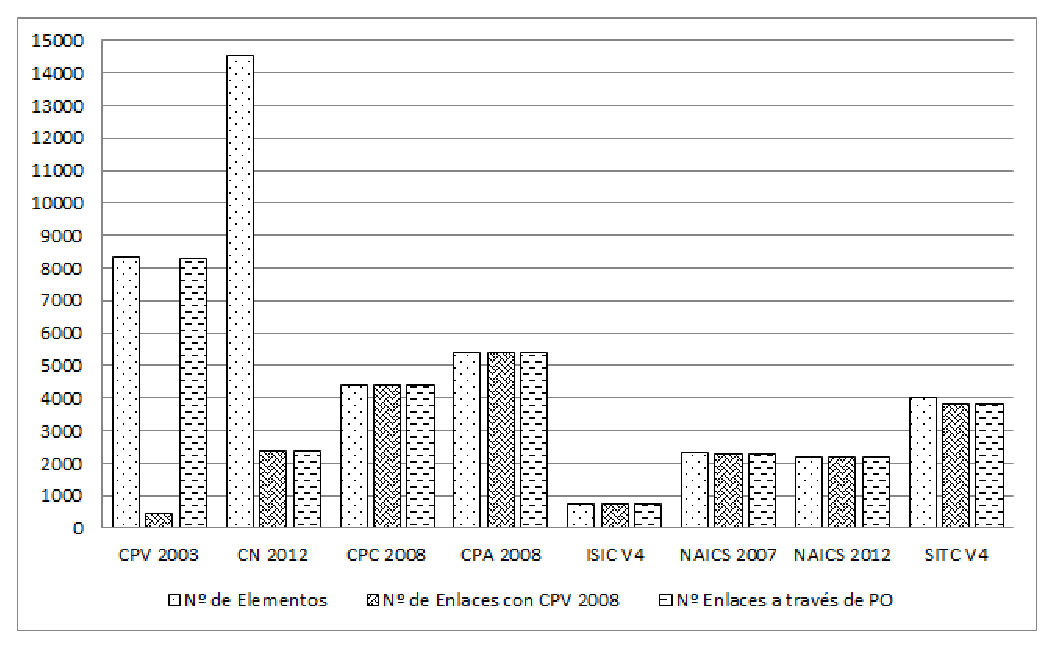
\includegraphics[width=14cm]{./images/phd/experimentation/pscs-enlaces}
\caption{Gráfica de Número de Elementos y Enlaces entre las PSCs y el CPV 2008.}
\label{fig:pscs-enlaces}
\end{figure}

\begin{figure}[!htb]
\centering
	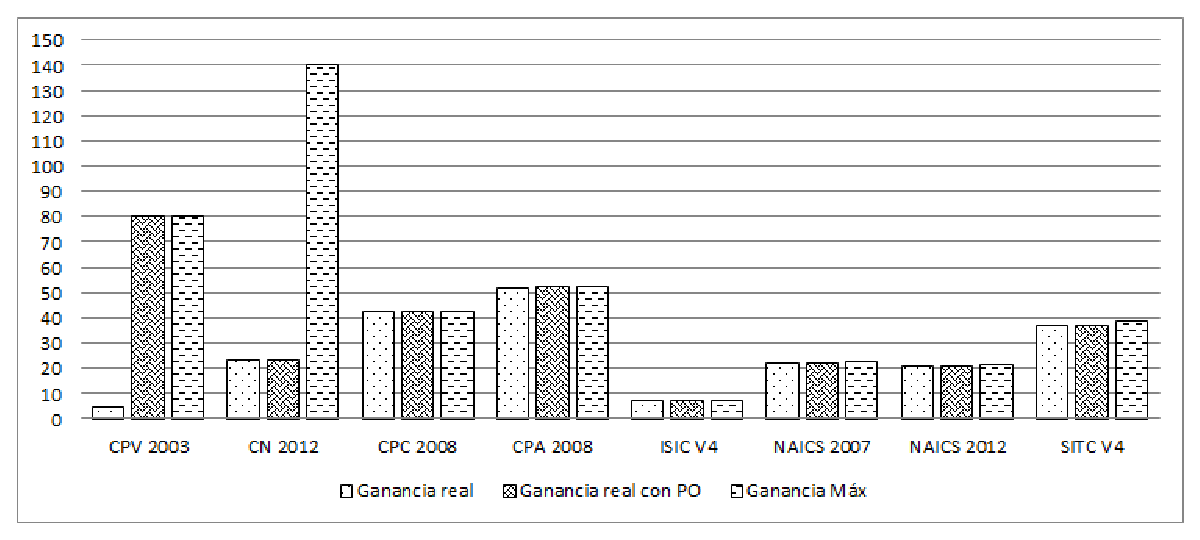
\includegraphics[width=14cm]{./images/phd/experimentation/pscs-ganancia}
\caption{Gráfica de Ganancia en expresividad.}
\label{fig:pscs-ganancia}
\end{figure}

\subsubsection{Punto de vista Cualitativo}
La ejecución de este experimento requiere la evaluación uno a uno de los criterios diseñados en las distintas 
tablas para su posterior evaluación. Para ello, se han acumulado en una hoja de cálculo las respuestas 
de cada uno de los enfoques y agregado todos los resultados en las Tablas~\ref{tabla:agregado-full} y~\ref{tabla:agregado-full-porcentaje}, 
también de forma gráfica en las Figuras~\ref{fig:eval-criteria-ppn},~\ref{fig:eval-criteria-pscs} y~\ref{fig:eval-criteria-orgs} se 
pueden observar los resultados obtenidos. De esta forma, se recoge por un lado 
la valoración y por otra la representación gráfica respecto al modelo de referencia. En el Apéndice~\ref{tablas-validacion-apen} se 
presenta la valoración para el modelo de referencia como ejemplo de evaluación y para la visualización del diseño de las 
tablas de validación.

\begin{sidewaystable}[ht!]
\renewcommand{\arraystretch}{1.3}
\begin{center}
\begin{tabular}{|p{3cm}||c|c|c||c|c|c||c|c|c||c|c|c||c|c|c||c|c|c||c|c|c||c|c|c|}
\hline
\textbf{Versión}&\multicolumn{3}{|c||}{$T^{1}$} & \multicolumn{3}{|c||}{$T^{2}$}& \multicolumn{3}{|c||}{$T^{3}$} & \multicolumn{3}{|c||}{$T^{3}_1$} & \multicolumn{3}{|c||}{$T^{4}$} & \multicolumn{3}{|c||}{$T^{4}_1$} & \multicolumn{3}{|c||}{$T^{5}$} & \multicolumn{3}{|c|}{$T^{6}$} \\ \hline
 &\si&\no&\na&	\si&\no&\na&	\si&\no&\na&	\si&\no&\na&	\si&\no&\na&	\si&\no&\na&	\si&\no&\na&	\si&\no&\na \\ \hline
 \textbf{Referencia} &\textbf{60}&\textbf{0}&\textbf{9}&	\textbf{44}&\textbf{0}&\textbf{0}&	\textbf{4}&\textbf{0}&\textbf{0}&	\textbf{5}&\textbf{0}&\textbf{0}&	\textbf{8}&\textbf{0}&\textbf{0}&	\textbf{14}&\textbf{0}&\textbf{0}&	\textbf{5}&\textbf{0}&\textbf{0}&	\textbf{33}&\textbf{0}&\textbf{14}\\ \hline \hline
  \multicolumn{25}{|c|}{\textbf{Anuncios de Licitación}} \\ \hline
 \textbf{\gls{TED}}	     			& 13 & 7 & 49 	& 0 & 0 & 44  	& 1 & 0 & 3  & 1 & 0 & 4  & 6 & 2 & 0  & 11 & 3 & 0  	& 0 & 0 & 5  & 0 & 0 & 47 \\ \hline
 \textbf{Plataforma de Contratación}	& 15 & 5 & 49 	& 0 & 0 & 44  	& 1 & 0 & 3  & 1 & 0 & 4  & 7 & 1 & 0  & 11 & 3 & 0  	& 0 & 0 & 5  & 0 & 0 & 47 \\ \hline 
 \textbf{\gls{BOE}}	     			& 10 & 9 & 50 	& 0 & 0 & 44  	& 1 & 0 & 3  & 1 & 0 & 4  & 8 & 0 & 0  & 10 & 3 & 1  	& 0 & 0 & 5  & 0 & 0 & 47 \\ \hline 
 \textbf{Servicios Externos}	     	& 12 & 8 & 49 	& 0 & 0 & 44  	& 1 & 0 & 3  & 1 & 0 & 4  & 5 & 3 & 0  & 6 & 3 & 5  	& 0 & 0 & 5  & 0 & 0 & 47 \\ \hline 
 \textbf{LOTED}	     			& 35 & 24 & 10 	& 23 & 8 & 13  	& 4 & 0 & 0  & 5 & 0 & 0  & 8 & 0 & 0  & 12 & 2 & 0  	& 5 & 0 & 0  & 0 & 0 & 47 \\ \hline 
 \textbf{\gls{MOLDEAS}}	     		& 54 & 7 & 8  	& 31 & 3 & 10 	& 4 & 0 & 0  & 5 & 0 & 0  & 8 & 0 & 0  & 14 & 0 & 0 	& 5 & 0 & 0  & 0 & 0 & 47 \\ \hline 
 \multicolumn{25}{|c|}{\textbf{Catálogo de Clasificaciones de Productos}} \\ \hline
 \textbf{\gls{CSV}/MSExcel} & 9 & 4 & 56 & 0 & 0 & 44 & 0 & 0 & 4 & 2 & 0 & 3 & 8 & 0 & 0 & 6 & 8 & 0 & 0 & 0 & 5 & 0 & 0 & 47 \\ \hline 
 \textbf{Servicios on-line} & 11 & 11 & 47 & 0 & 0 & 44 & 0 & 0 & 4 & 0 & 0 & 5 & 5 & 2 & 1 & 5 & 8 & 1 & 0 & 0 & 5 & 0 & 0 & 47 \\ \hline 
 \textbf{\gls{MOLDEAS}}& 54 & 7 & 8 & 31 & 3 & 10 & 4 & 0 & 0 & 5 & 0 & 0 & 8 & 0 & 0 & 14 & 0 & 0 & 5 & 0 & 0 & 32 & 0 & 15 \\ \hline 
 \multicolumn{25}{|c|}{\textbf{Organizaciones}} \\ \hline
 \textbf{TED} 			&  3 & 3 & 63 & 0 & 0 & 44 & 0 & 0 & 4 & 1 & 0 & 4 & 6 & 2 & 0 & 10 & 4 & 0 & 0 & 0 & 5 & 0 & 0 & 47 \\ \hline 
 \textbf{Plataforma de Contratación} &    13 & 4 & 52 & 0 & 0 & 44 & 1 & 0 & 3 & 1 & 4 & 0 & 8 & 0 & 0 & 12 & 2 & 0 & 0 & 0 & 5 & 0 & 0 & 47 \\ \hline 
 \textbf{\gls{BORME}}			 &    1 & 0 & 68 & 0 & 0 & 44 & 0 & 0 & 4 & 1 & 0 & 4 & 8 & 0 & 0 & 13 & 1 & 0 & 0 & 0 & 5 & 0 & 0 & 47 \\ \hline 
 \textbf{Servicios Externos} 	&  12 & 8 & 49 & 0 & 0 & 44 & 1 & 0 & 3 & 1 & 0 & 4 & 1 & 7 & 0 & 5 & 5 & 4 & 0 & 0 & 5 & 0 & 0 & 47 \\ \hline 
 \textbf{\gls{BBDD} externa} 		&     1 & 0 & 68 & 0 & 0 & 44 & 0 & 0 & 4 & 0 & 0 & 5 & 1 & 5 & 2 & 10 & 4 & 0 & 0 & 0 & 5 & 0 & 0 & 47 \\ \hline 
 \textbf{OpenCorporates} 	&    35 & 22 & 12 & 21 & 10 & 13 & 4 & 0 & 0 & 4 & 0 & 1 & 8 & 0 & 0 & 13 & 1 & 0 & 0 & 0 & 5 & 0 & 0 & 47 \\ \hline 
 \textbf{MOLDEAS} 		&    54 & 7 & 8 & 44 & 0 & 0 & 4 & 0 & 0 & 5 & 0 & 0 & 8 & 0 & 0 & 14 & 0 & 0 & 5 & 0 & 0 & 0 & 0 & 47 \\ \hline 
\hline
  \end{tabular}
  \caption{Tabla agregada de Validación Conjunta con Valores Parciales.}
  \label{tabla:agregado-full}
  \end{center}
\end{sidewaystable} 

\cleardoublepage

\begin{figure}[!htb]
\centering
	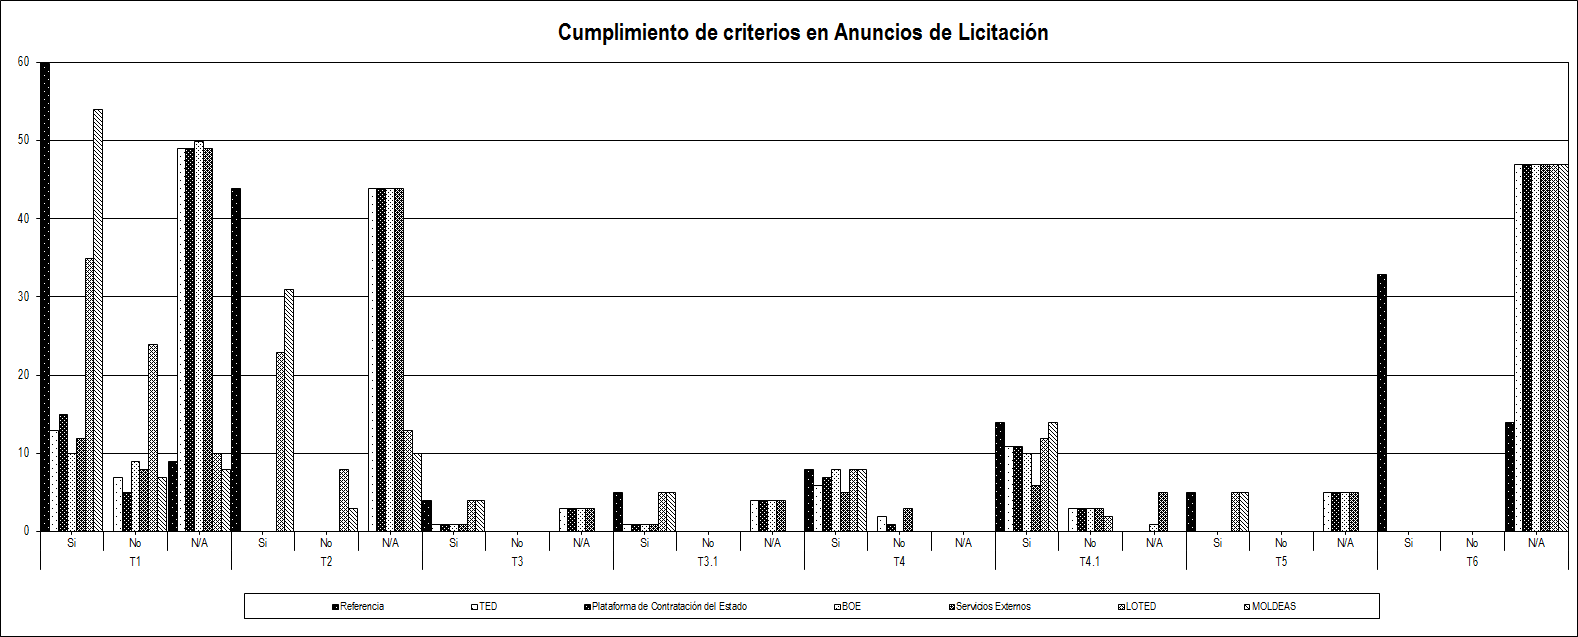
\includegraphics[width=16cm]{./images/phd/experimentation/criterios-ppn}
\caption{Gráfica del Grado de Cumplimiento de Criterios en Anuncios de Licitación.}
\label{fig:eval-criteria-ppn}
\end{figure}

\begin{figure}[!htb]
\centering
	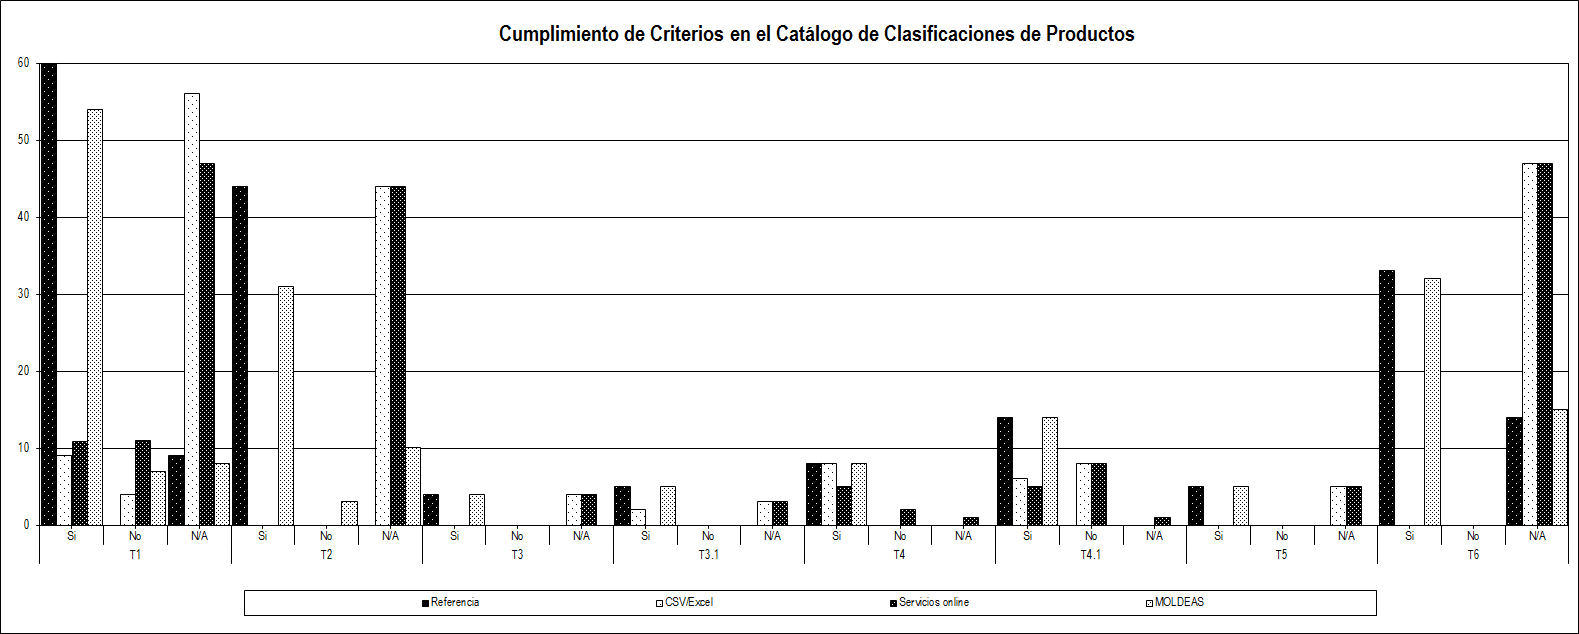
\includegraphics[width=16cm]{./images/phd/experimentation/criterios-pscs}
\caption{Gráfica del Grado de Cumplimiento de Criterios en el Catálogo de Clasificaciones de Productos.}
\label{fig:eval-criteria-pscs}
\end{figure}

\begin{figure}[!htb]
\centering
	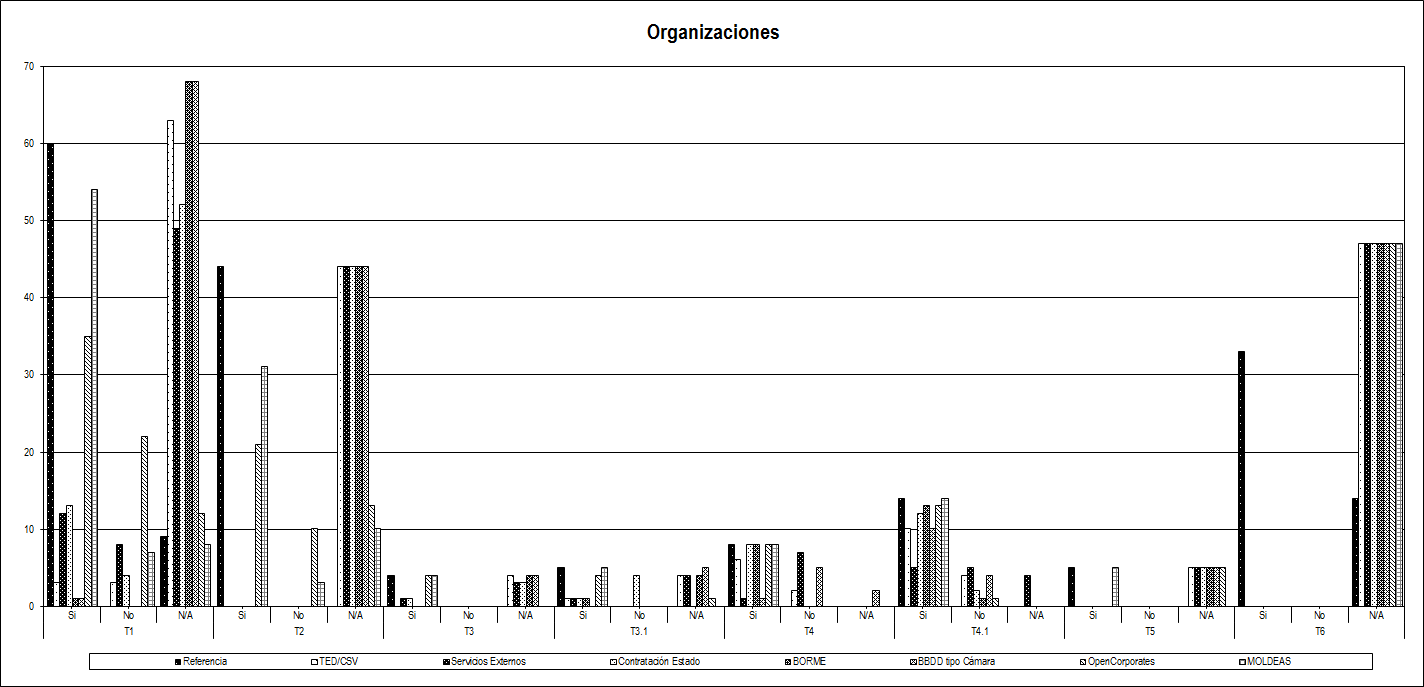
\includegraphics[width=16cm]{./images/phd/experimentation/criterios-orgs}
\caption{Gráfica del Grado de Cumplimiento de Criterios en las Organizaciones.}
\label{fig:eval-criteria-orgs}
\end{figure}

En la Tabla~\ref{tabla:agregado-sumatorio} se presenta la suma de todos los criterios para cada una de las tablas de validación, con el 
objetivo de ofrecer una visión simplificada de la evaluación. Con el objetivo de representar esta información de forma 
gráfica y poder realizar una comparación visual se han elaborado las siguientes gráficas tanto para los 
anuncios de licitación, ver Figura~\ref{fig:eval-criteria-1-ppn}, como para el catálogo de clasificaciones de productos, ver Figura~\ref{fig:eval-criteria-1-ppn}, y 
finalmente para la información y datos relativos a las organizaciones, ver Figura~\ref{fig:eval-criteria-1-orgs}.


\begin{longtable}[c]{|p{3cm}|c|c|c|c|c|c|c|c|}
\hline
\textbf{Versión}&$T^{1}$ & $T^{2}$& $T^{3}$ & $T^{3}_1$ & $T^{4}$ & $T^{4}_1$ &$T^{5}$ & $T^{6}$ \\ \hline
\endhead
 \multicolumn{9}{|c|}{\textbf{Anuncios de Licitación}} \\ \hline
 \textbf{TED}	     			& $65$ & \na & $100$ & $100$ & $75$ & $78,57$ & \na & \na \\ \hline
 \textbf{Plataforma de Contratación}	& $75$ & \na & $100$ & $100$ & $87,5$ & $78,57$ & \na & \na \\ \hline 
 \textbf{BOE}	     			& $52,63$ & \na & $100$ & $100$ & $100$ & $76,92$ & \na & \na\\ \hline 
 \textbf{Servicios Externos}	     	& $60$ & \na & $100$ & $100$ & $62,5$ & $66,66$ & \na & \na \\ \hline 
 \textbf{LOTED}	     			& $59,32$ & $74,19$ & $100$ & $100$ & $100$ & $85,71$ & $100$ & \na \\ \hline 
 \textbf{MOLDEAS}	     		& $88,52$ & $91,18$ & $100$ & $100$ & $100$ & $100$ & $100$ & \na \\ \hline 
 \multicolumn{9}{|c|}{\textbf{Catálogo de Clasificaciones de Productos}} \\ \hline
 \textbf{CSV/MSExcel} 			&$69,23$ & \na & \na & $100$ & $100$ & $42,86$ & \na & \na \\ \hline 
 \textbf{Servicios on-line}  		&$50$ & \na & \na & \na & $71,43$ & $38,46$ & \na & \na \\ \hline 
 \textbf{MOLDEAS}			&$88,52$ & $100$ & $100$ & $100$ & $100$ & $100$ & $100$ & $100$ \\ \hline 
 \multicolumn{9}{|c|}{\textbf{Organizaciones}} \\ \hline
 \textbf{TED} 				& $50$ & \na & \na & $100$ & $75$ & $71,43$ & \na & \na \\ \hline 
 \textbf{Plataforma de Contratación} 	& $76,47$ & \na & $100$ & $20$ & $100$ & $85,71$ & \na & \na\\ \hline 
 \textbf{BORME}			 	& $100$ & \na & \na & $100$ & $100$ & $92,85$ & \na & \na \\ \hline 
 \textbf{Servicios Externos} 		& $60$ & \na & $100$ & $100$ & $12,5$ & $50$ & \na & \na \\ \hline 
 \textbf{BBDD externa} 			& $100$ & \na & \na & \na & $16,67$ & $71,43$ & \na & \na \\ \hline 
 \textbf{OpenCorporates} 	 	& $61,40$ & $67,74$ & $100$ & $100$ & $100$ & $92,86$ & $100$ & \na\\ \hline 
 \textbf{MOLDEAS} 		 	& $88,52$ & $91,18$ & $100$ & $100$ & $100$ & $100$ & $100$ & \na \\ \hline 
\hline
  \caption{Tabla agregada de Validación Conjunta con Porcentajes \si entre aplicables.}
  \label{tabla:agregado-full-porcentaje}
\end{longtable} 



\begin{longtable}[c]{|l|c|c|c||c||c|} 
\hline
 \textbf{Versión} & \si&\no&\na & \textbf{Total} & \textbf{\% \si entre aplicables} \\\hline
\endhead
    \textbf{Referencia} & 173 & 0 & 23 & 196& 100 \\ \hline \hline
 \multicolumn{6}{|c|}{\textbf{Anuncios de Licitación}} \\ \hline   
     \textbf{TED} & 32 & 12 & 152 &$\equiv$ & $72.72$\\ \hline 
     \textbf{Plataforma de Contratación} & 35 & 9 & 152 &$\equiv$ & $79.54$\\ \hline 
    \textbf{BOE} & 30 & 12 & 154 &$\equiv$ & $71.42$\\ \hline 
    \textbf{Servicios Externos} & 25 & 14 & 157 &$\equiv$ & $64.10$\\ \hline 
    \textbf{LOTED} & 92 & 34 & 70 &$\equiv$ & $73.01$\\ \hline 
     \textbf{MOLDEAS} & 121 & 10 & 65 &$\equiv$ & $92.36$\\ \hline 
 \multicolumn{6}{|c|}{\textbf{Catálogo de Clasificaciones de Productos}} \\ \hline
    \textbf{CSV/MSExcel} &  25 & 12 & 159 &$\equiv$ & $67.56$\\ \hline 
     \textbf{Servicios on-line} &  21 & 21 & 154 &$\equiv$ & $50$\\ \hline 
    \textbf{MOLDEAS} &  166 & 7 & 23 &$\equiv$ & $93.86$\\ \hline 
 \multicolumn{6}{|c|}{\textbf{Organizaciones}} \\ \hline
    \textbf{TED} & 20 & 9 & 167 &$\equiv$ & $68.96$\\ \hline 
    \textbf{Plataforma de Contratación}  & 35 & 10 & 151 &$\equiv$ & $77.77$ \\ \hline 
    \textbf{BORME}  & 23 & 1 & 172 &$\equiv$ & $95.83$\\ \hline 
    \textbf{Servicios Externos}  & 20 & 20 & 156 &$\equiv$ & $50$\\ \hline   
    \textbf{BBDD externa}  & 12 & 9 & 175 &$\equiv$ & $57.14$\\ \hline 
    \textbf{OpenCorporates}  & 85 & 33 & 78  &$\equiv$ & $72.03$\\ \hline 
    \textbf{MOLDEAS}  & 121 & 10 & 65 &$\equiv$ & $92.36$\\ \hline 
\hline
\caption{Tabla agregada de Validación Conjunta con Valores Totales.}\label{tabla:agregado-sumatorio}\\    
\end{longtable}

\cleardoublepage

\begin{figure}[!htb]
\centering
	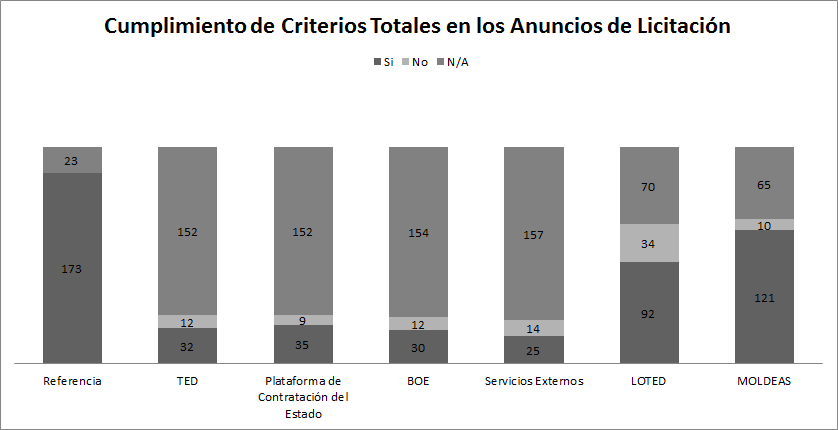
\includegraphics[width=12cm]{./images/phd/experimentation/criterios-total-ppn}
\caption{Gráfica del Grado de Cumplimiento Total de Criterios en Anuncios de Licitación.}
\label{fig:eval-criteria-1-ppn}
\end{figure}

\begin{figure}[!htb]
\centering
	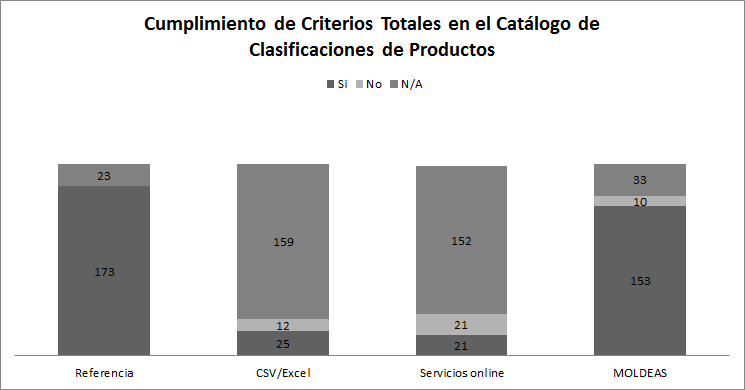
\includegraphics[width=14cm]{./images/phd/experimentation/criterios-total-pscs}
\caption{Gráfica del Grado de Cumplimiento Total de Criterios en el Catálogo de Clasificaciones de Productos.}
\label{fig:eval-criteria-1-pscs}
\end{figure}

\begin{figure}[!htb]
\centering
	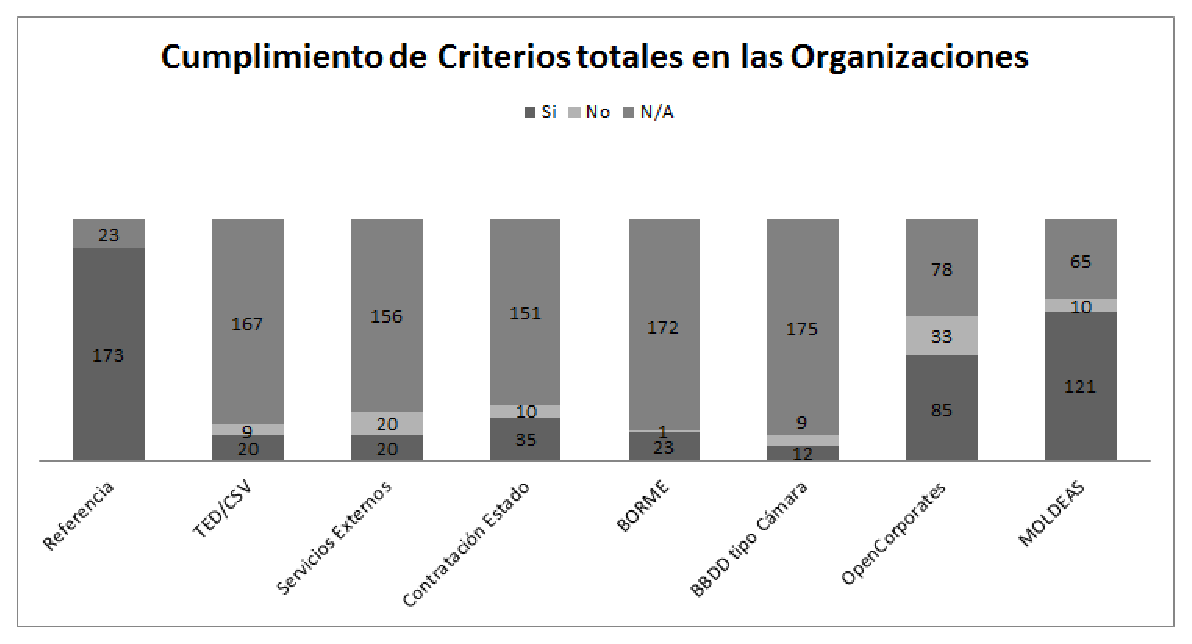
\includegraphics[width=14cm]{./images/phd/experimentation/criterios-total-orgs}
\caption{Gráfica del Grado de Cumplimiento Total de Criterios en las Organizaciones.}
\label{fig:eval-criteria-1-orgs}
\end{figure}


\subsection{Validación del experimento sobre la aplicación de \textit{Linked Data} a las Licitaciones Públicas}\label{sect:validation-tablas}


\subsubsection{Punto de vista Cuantitativo}\label{sect:experimento-pscs-validation}
El experimento diseñado y probado permite la verificación del porcentaje de ganancia al añadir y enlazar un vocabulario 
controlado con el \gls{CPV} 2008. La validación de este experimento debe plantearse asumiendo las siguientes premisas:
\begin{itemize}
 \item La selección del CPV 2008 como vocabulario matriz para el acceso a los anuncios de licitación pública 
en el ámbito de la Unión \gls{Europea}.
\item La condición de que todos los anuncios de licitación pública deben estar etiquetados obligatoriamente con 
este vocabulario.
\item La restricción de que el número de términos en el CPV 2008 es limitado.
\item La diferencia de recuperación de información entre un sistema basado en texto libre en contraposición con los 
basados en un vocabulario controlado.
\item La diversificación de vocabularios controlados, taxonomías, etc., existentes para el etiquetado de productos 
y servicios en diferentes ámbitos y con objetivos dispares: trazabilidad, extracción de estadísticas, etc.
\item La necesidad de realizar una combinación efectiva entre las clasificaciones de productos para asegurar
la comparación entre los mismos.
\item El número de documentos recuperados es completo si se utiliza todo el vocabulario del CPV 2008.
\end{itemize}

Bajo estas condiciones, el paradigma basado en \linkeddata permite que, a través de una correcta aplicación 
de un ciclo de vida para la generación de las clasificaciones de productos en \gls{RDF} y su enlazado posterior, 
se suministre el soporte necesario para cumplir con las premisas fijadas aumentando la capacidad expresiva 
del vocabulario de entrada para la recuperación de información de los anuncios de licitación pública en el 
ámbito europeo aumentando así la capacidad expresiva de los posibles clientes.

Desde el punto de vista del análisis de los resultados obtenidos y señalados en la sección anterior mediante la 
Tabla~\ref{ganancia-terminos} se pueden extraer las siguientes puntos clave:
\begin{itemize}
 \item La ganancia máxima ideal de expresividad se obtendrá cuando el vocabulario a añadir al conjunto de entrada 
contenga el mayor número de términos, es el caso de la clasificación de productos CN 2012. 
No obstante, el porcentaje de ganancia real dependerá siempre del número de términos que han sido enlazados 
al vocabulario matriz, en este caso el CPV 2008.
\item Hay que tener en cuenta que los enlaces generados desde una clasificación al CPV 2008 se encuentran 
bajo un umbral $\mu$ según el cual se admite la creación del enlace entre un concepto de una clasificación 
y el CPV 2008. Este umbral puede variar de una aplicación a otro y dependiendo del sistema de reconciliación 
de entidades utilizado será más o menos exacto. El objetivo reside en que la posibilidad de aumentar el vocabulario 
de entrada pudiendo realizar consultas bajo un determinado umbral $mu$ de concreción del enlace.
\item De todos los enlaces generados entre las clasificaciones de productos y el CPV 2008 $1503+462 = 1965$ son exactos 
porque han sido realizados por fuentes oficiales. Esto supone un incremento del $8.65\%$ y $6.64\%$ (a través de \textit{ProductOntology}) 
 en el número de términos nuevos posibles en el vocabulario de entrada perfectamente enlazados sin ningún umbral de ambig\"{u}edad, 
simplemente realizando su transformación a \linkeddata y creando los enlaces entre sí de forma automática. Los porcentajes 
restantes de $91.35\%$ y $93.36\%$ respectivamente indican enlaces automáticos, esta situación es habitual en el ámbito 
de \linkeddata y la única forma de decrementar estos valores consiste en la intervención manual para la validación 
de los enlaces con expertos del dominio.
\item Respecto a la ganancia en términos porcentuales se fija un máximo de $405.86\%$, un real $209.66\%$ y un real a través 
de \textit{ProductOntology} de $285.66\%$, lo que supone respectivamente un incremento de la expresividad de $5$, $3$ y cerca de 
$4$ veces más, en el número de nuevos términos a utilizar en el vocabulario de entrada debido al uso de \linkeddata respecto 
a la versión actual.
\item La selección de una nueva clasificación para ser enlazada con el CPV 2008 se debería basar en los siguientes criterios:
\begin{enumerate}
 \item Número de términos.
 \item Ganancia ideal y real.
\end{enumerate}

No obstante, se establece un nuevo parámetro consistente en el número de enlaces exactos que se pueden establecer 
entre el vocabulario a añadir y el matriz, facilitando así la comprobación de la calidad de la adición del nuevo 
vocabulario. Esta situación pese a que responde a un entorno ideal, la realidad es que en el ámbito de datos enlazados 
se trabaja bajo unos ciertos umbrales de incertidumbre que son admitidos por la propia comunidad. Evidentemente, dependiendo 
del tipo de aplicación este punto debe ser considerado en mayor o menor medida.

\item En cuanto al uso de un vocabulario intermedio como es \textit{ProductOntology} su uso se convierte en estratégico 
por su carácter internacional. En general, no existe una mejora excesivamente reseñable respecto al enlazado de términos 
directo o indirecto salvo en el CPV 2003, en el cual sólo se habían contemplado los enlaces exactos, y que supone 
un incremento del número de términos enlazados desde el $4.46 \%$ al $80.25 \%$. Esto implica que el proceso de enlazado inicial 
entre una clasificación y el CPV 2008 ha sido lo suficientemente bueno como para no ser necesario un paso intermedio mediante 
otro vocabulario que pudiera realizar el descubrimiento de nuevos enlaces.

\item Respecto al enlazado entre el \gls{CPV} 2008 y \textit{ProductOntology} si bien supone una ganancia apreciable en cuanto 
a expresividad de entrada, $10000$ nuevos términos posibles, simplemente se ha implementado y señalado pero no se considera estrictamente 
adecuado aunque aumente considerablemente la expresividad, ya que el vocabulario de entrada posible de \textit{ProductOntology} es $\inf$ por construcción del mismo, 
por lo que se prefiere su uso como puente entre una \gls{PSC} y el CPV 2008 y no se compara con las demás clasificaciones de productos en cuanto 
a características: vocabulario controlado, realizado por una entidad, etc.

\item Finalmente, es conveniente tener presente el problema de la recursión y posibilidad de convertir un vocabulario 
controlado de entrada (finito) en infinito por la suposición de nuevos enlaces entre elementos que directamente 
no están enlazados. Esta cuestión es perjudicial en dominios concretos y cerrados, como en el caso de los anuncios 
de licitación pública europea, pero si es beneficiosa (o admisible) en un entorno abierto para la realización de consultas 
de extracción de información sobre una base de datos infinita como es la Web, siempre teniendo presente el tiempo 
de la federación de consultas, etc., como se ha presentando en secciones anteriores

\end{itemize}

\subsubsection{Punto de vista Cualitativo}
El experimento y evaluación realizada permiten realizar una calificación y comparación entre los distintos enfoques 
disponibles para la publicación y acceso a la información y datos referente a los anuncios de licitación, incluyendo
el catálogo de clasificaciones de productos y las organizaciones. El diseño de las tablas, como se ha señalado, busca 
la valoración de criterios correspondientes a la iniciativa \linkeddata y \opendata. De esta forma, si las valoraciones 
son completas en términos de valores positivos para las Tablas $T^{3}$, $T^{3}_1$ y $T^{4}$ se puede asegurar 
que los datos evaluados cumplen todos los criterios para ser considerados datos enlazados y abiertos, además 
de situarse con la máxima valoración en el modelo de 5 $\star$. Teniendo en cuenta esta premisa, aquellos 
enfoques que se sitúen bajo estas premisas estarán facilitando el acceso a la información de los anuncios 
de licitación mediante la aplicación completa de estas iniciativas y por lo tanto, se puede asegurar que 
todos los beneficios y ventajas que se proponen bajo estos paradigmas se cumplen, por ejemplo los presentados en la Tabla $T^{4}_1$. Además de este valoración 
principal de los criterios de \linkeddata y \opendata se han propuesto otras tablas con el objetivo de 
validar la calidad de los datos producidos en el sentido de la información y metainformación que contienen, 
el modelo de producción y publicación utilizado y las facilidades de consumo de los datos suministradas, estas 
características se ven reflejadas en la Tabla $T^{1}$. Adicionalmente y al igual que en el diseño del \textit{software}, 
es conveniente la aplicación de patrones de diseño con el objetivo de resolver problemas comunes mediante un enfoque 
sistemático, esta cuestión conlleva la valoración de los patrones de diseño utilizados al modelar los datos enlazados y que 
se propone en la Tabla $T^{2}$. Finalmente, como uno de los puntos de clave para la difusión de los datos enlazados y 
cumpliendo la motivación inicial de esta iniciativa de reutilización de información, es importante la validación en 
cuanto a la posibilidad de pertenencia a la nube de datos enlazados, Tabla $T^{5}$, así como a los registros CKAN, Tabla $T^{6}$. Si 
bien los criterios de estas últimas tablas no son obligatorios en el sentido de \linkeddata, si que tienen una importancia 
capital cuando nos referimos a datos enlazados abiertos, ya que carece de sentido realizar un esfuerzo para la apertura 
y enlazado de datos si la meta final no reside en su posterior reutilización. 

A continuación se realiza una validación pormenorizada para cada uno de los conjunto de datos y enfoques 
evaluados, se ha agrupada la valoración respecto a las tablas realizadas ya que la justificación de los resultados 
es similar en cada uno de los conjuntos de datos:

\begin{enumerate}
 \item Atendiendo a las calificaciones de cada uno de los enfoques se puede observar 
como varios de los enfoques tienen características propias de los procesos implicados en la iniciativa de 
\linkeddata en cuanto a la publicación de datos y el diseño del acceso a la información a través de \gls{URI}s, de ahí 
que los distintos enfoques obtengan ciertos criterios positivos en la Tabla $T^{1}$ pese a que no se consideren
bajo el paradigma de datos enlazados. Sin embargo, el esfuerzo realizado en el proyecto LOTED se ve reflejado 
en un grado aceptable de cumplimiento de los criterios evaluados, la negatividad de otros queda justificada por la 
ausencia de metainformación en los \datasets. En el caso particular del enfoque propuesta por este trabajo, \gls{MOLDEAS}, 
las calificaciones son positivas en un grado muy alto debido a la aplicación de un ciclo de vida para la generación 
de datos enlazados como un proceso de ingeniería, no obstante los puntos negativos obtenidos se refieren a cuestiones 
relacionadas con la documentación adicional necesaria que debería ser labor del experto en el dominio y dirigida 
a diferentes usuarios (técnicos, finales, etc.).

\item En cuanto a la validación de acuerdo a los patrones de diseño presentes en la Tabla $T^{2}$, los enfoques que utilizan datos enlazados si reflejan 
la aplicación de los mismos, si bien no se considera necesario la aplicación de todos ellos, si es conveniente 
aplicarlos en la mayor medida posible. 

\item De nuevo la Tablas $T^{3}$, $T^{3}_1$ van dirigidas a los enfoques basados en datos enlazados principalmente, por lo que 
aquellos esfuerzos que no se encuentran bajo esta paradigma resultan ampliamente damnificados en su evaluación, cubriendo 
tan sólo alguna características básica. 

\item Sin embargo, la calificación de casi todos los enfoques en lo referente a los principios
de \opendata en la Tablas $T^{4}$, $T^{4}_1$ es verdaderamente positiva debido principalmente a la naturaleza de la información 
y datos que es intrínsecamente abierta. Aquellos enfoques que ofrecen servicios de negocios se ven penalizados debido a que 
utilizan datos abiertos pero su estrategia o política posterior con los mismos restringe su uso y tan sólo cumplirán estos 
requisitos si los servicios de suscripción fueran libres respecto a la información, manteniendo su coste respecto al servicio 
construido sobre los datos, por ejemplo análisis, predicción o estadísticas. Evidentemente, esta situación sería ideal y también 
deben obtener rentabilidad del coste de recuperación de información.

\item Las Tablas $T^{5}$, $T^{6}$ son orientadas nuevamente a las iniciativas basadas en datos enlazados ya que carecen 
de sentido para las demás debido a su naturaleza. En este sentido, tanto los enfoques realizados por MOLDEAS y LOTED son 
candidatos a pertenecer a la nube de datos enlazados y a los registros \gls{CKAN} sin ningún tipo de inconveniente.

\end{enumerate}

En general, la tendencia que se observa en las tablas es que la información y datos relativa a los anuncios de licitación, 
clasificaciones de productos y organizaciones tiene un carácter abierto, como confirman los resultados, e incluso disponen
de buenos fundamentos para que la realización del esfuerzo de transformación a datos enlazados sea asumible tanto 
por las Administraciones Públicas como por terceros, así lo demuestra el trabajo presentado en este documento 
a través del enfoque realizado en \gls{MOLDEAS}. La aplicación de los principios de \linkeddata y \opendata permiten 
asegurar ventajas y beneficios en el acceso a la información y manejo de los datos tanto para las personas físicas 
como para los componentes software, facilitando su consumo y permitiendo impulsar la creación de nuevos servicios 
de valor añadido con la información relevante de los anuncios de licitación y su entorno. De esta manera, el esfuerzo 
realizado por las empresas actuales de recuperar información de fuentes de datos heterogéneas y con distintos 
formatos como \gls{PDF}, \gls{HTML}, etc., es altamente mitigado debido al uso de datos enlazados.

\subsection{Evaluación del experimento sobre la aplicación de \textit{Linked Data} a las Licitaciones Públicas}


\subsubsection{Punto de vista Cuantitativo}
La ejecución y validación del experimento del uso de datos enlazados en la recuperación de información de 
los anuncios de licitación aumentando la expresividad del vocabulario de entrada (\gls{CPV} 2008) permite 
dar respuesta las preguntas establecidas en el diseño del experimento.

\begin{itemize}
 \item ¿Cuál es la expresividad actual, en términos de número de conceptos para realizar consultas, 
para el acceso a la información de anuncios de licitación?

La versión inicial y los sistemas disponibles en Internet hacen uso del vocabulario CPV 2008 para la creación de consultas 
sobre los anuncios de licitación disponiendo de una expresividad como vocabulario de entrada de $10357$ términos. Debido 
a que este vocabulario es normativo a nivel europeo en el sentido de que cualquier anuncio de licitación debe 
contener al menos un código CPV 2008, se puede establecer que utilizando el conjunto completo de términos del vocabulario 
de entrada se puede acceder a la base documental completa de los anuncios de licitación, independientemente de la tecnología 
utilizada.

\item ¿Cuál es la ventaja de uso de un modelo \gls{RDF} para la expresión y recuperación de la información de los anuncios de licitación?

Además de las ventajas intrínsecas del uso de RDF y la realización práctica del enfoque de \linkeddata sobre las clasificaciones 
de productos y la información de los anuncios de licitación pública europea, el principal beneficio reside en el enlazado de datos 
desde otro vocabulario de entrada al CPV 2008 permitiendo el incremento el número de términos del vocabulario de entrada que inicialmente 
sólo contiene a los términos del CPV 2008 y mediante esta técnica se incrementa notablemente, aumentando el universo del discurso para 
la recuperación de información de los anuncios de licitación. 

 \item ¿Cómo los datos enlazados favorecen el aumento de expresividad en la ejecución de consultas y por tanto facilitan la recuperación de los 
anuncios de licitación? 

Según la respuesta realizada en la pregunta anterior y la validación presentada en la Sección~\ref{sect:experimento-pscs-validation}, el uso 
de datos enlazados beneficia la creación de consultas enriquecidas respecto al vocabulario de entrada permitiendo al cliente la utilización 
de un mayor número de términos convirtiendo el conocimiento del CPV 2008 en opcional. En la validación realizada y con la transformación 
de las clasificaciones de productos realizadas se obtiene un incremento entre $3$ y $4$ veces más respecto al 
número de términos posibles iniciales provenientes del CPV 2008, la evolución del número de términos se puede observar en 
la Figura~\ref{fig:eval-n-terminos}.

\begin{figure}[!htb]
\centering
	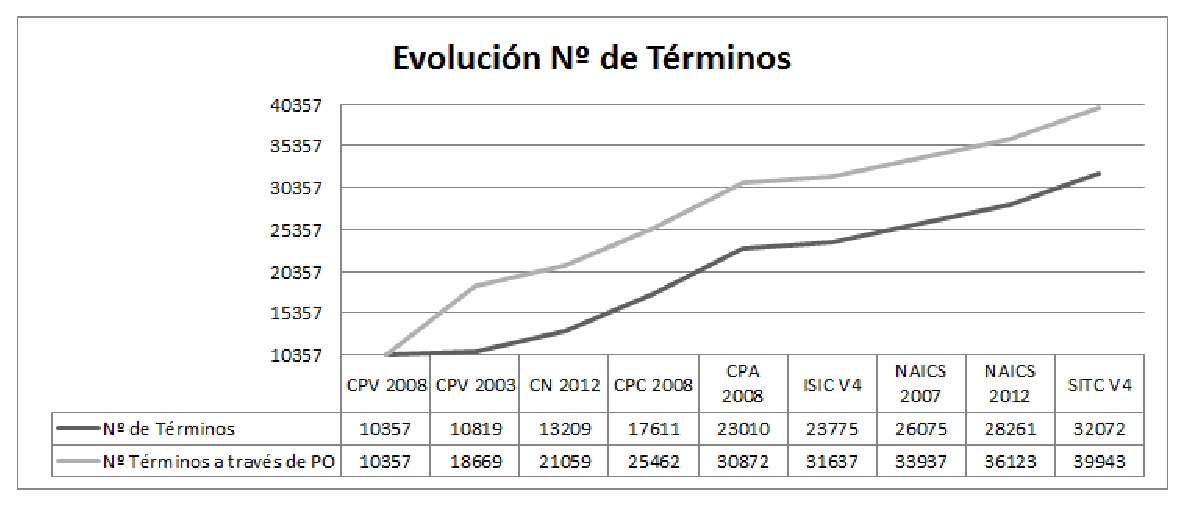
\includegraphics[width=14cm]{./images/phd/experimentation/evo-n-terminos}
\caption{Evolución Número de Términos.}
\label{fig:eval-n-terminos}
\end{figure}



\item ¿Cuál es el beneficio real del uso de datos enlazados para representar la información? 

El beneficio real reside en la representación de información y datos mediante un modelo estándar (\gls{RDF}) que permite el uso 
de lenguajes (\gls{SPARQL}) y protocolos (\gls{HTTP}) estándar para su acceso facilitando la recuperación de información. Evidentemente, 
el contraste respecto a las actuales versiones en \gls{HTML}, \gls{PDF}, MSExcel, etc., y sistemas de recuperación opacos suministradores 
por proveedores que generan servicios de negocio sobre ellos, es crítico, ya que simplemente el manejo de información 
de distintas fuentes y formatos requiere un esfuerzo que se solventa en gran medida con el uso de datos enlazados. Es necesario 
resaltar que el enfoque realizado en este documento es posible debido a la posibilidad de utilizar \opendata y mejorar éstos 
con la iniciativa de \linkeddata. Adicionalmente, se estable una fórmula para el cálculo de la ganancia al introducir 
una nueva clasificación enlazada con el \gls{CPV} 2008.

\item ¿Se incurre en algún error al aumentar la expresividad?

El enlazado de datos consta de una variable de incertidumbre que si bien es aceptada por la comunidad, debe ser tenida en cuenta 
para la realización de aplicaciones de carácter crítico. En este sentido y siguiendo con la validación realizada, al menos, 
se obtiene un incremento entre el $6.64\%$ (con \textit{ProductOntology}) y $8.65\%$ exacto del vocabulario controlado 
de entrado. En el caso particular de recuperación de documentos estos porcentajes son muy relevantes pero incluso 
la introducción de términos ``relacionados'' bajo un umbral de incertidumbre es conveniente ya que el funcionamiento 
del sistema se mantiene y se aumenta la expresividad de entrada para la realización de consultas. Por todo ello, 
pese a que este problema de enlazado de recursos y reconciliación de entidades está asociado a la iniciativa de 
\linkeddata, sólo se puede solventar con el esfuerzo de expertos en el dominio con el consiguiente coste. 

\end{itemize}

En resumen, el enfoque seguido en este experimento y en el estudio de este documento es extrapolable a un entorno o dominio en el cual exista un vocabulario 
controlado para la recuperación de documentos, existan diferentes vocabularios provenientes de distintas fuentes 
candidatos a interoperar con el inicial y en consecuencia a servir para el aumento del universo de discurso en 
ese dominio.


\subsubsection{Punto de vista Cualitativo}
La ejecución y validación del experimento del grado de cumplimento de criterios referentes a datos enlazados abiertos permite 
dar respuesta a las preguntas planteadas en el diseño del experimento.

\begin{itemize}
 \item ¿El ciclo de vida seguido y los datos generados certifican la aplicación de buenas prácticas de \linkeddata?

A la vista de la evaluación realizada de los distintos enfoques ha quedado patente que en la actualidad tanto la información 
como los datos disponibles son abiertos en su mayor parte e incluso son utilizados para la construcción de servicios 
comerciales pero el esfuerzo requerido para llevar a cabo estos productos se ve reflejado en el precio de los mismos. La aplicación 
de los principios de \linkeddata puede rebajar ampliamente este coste de acceso a la información promoviendo la 
competitividad y creando una administración más transparente. En este sentido el trabajo realizado en \gls{MOLDEAS} partiendo 
de la definición de un ciclo de vida (procesos, métodos y tareas) y del conjunto de datos referente al dominio de 
\eproc permite asegurar los criterios de \linkeddata además de cumplir las características más 
deseables en cuanto producción, publicación y consumo de datos.

 \item ¿El ciclo de vida seguido y los datos generados certifican el cumplimiento de los principios de \opendata?

De la misma forma que en la pregunta anterior el modelo de ciclo de vida seguido ha permitido conservar el carácter 
de datos abiertos intrínseco la información y datos relativa al entorno de los anuncios de licitación como se ha reflejado 
en las tablas de validación referentes a \opendata.

 \item ¿Qué nivel del modelo de 5 $\star$ se puede establecer?

Consecuentemente por la aplicación del ciclo de vida y las valoraciones realizadas en los criterios relativos al nivel 
dentro del modelo de 5 $\star$ se refleja la consecución de la calificación más alta. En este punto cabe realizar una reflexión 
sobre el nivel de estrellas que deben tener los datos abiertos enlazados, especialmente los referentes a las Administraciones Públicas. En muchos 
casos y especialmente desde un punto de vista de un desarrollados es suficiente la publicación de datos a través de \gls{RSS} (3 $\star$), esta situación 
es consecuencia directa de la simplicidad de este formato tanto en representación como por su madurez, ahora bien, la publicación de datos 
bajo 5 $\star$ confiere nuevas cualidades a los mismos como un modelo formal subyacente, la posibilidad de reconciliación automática, realización 
de procesos de razonamiento, etc., que para aplicaciones de gestión de la información avanzada resultan de gran interés. En conclusión, 
desde un punto de vista práctico el nivel de 3 $\star$ sería suficiente pero las ventajas adicionales de los datos 5 $\star$ debe conducir 
a una valoración por parte de los propietarios de datos a exigir este nivel aunque el esfuerzo inicial sea mayor la recompensa a medio/largo 
plazo debe ser superior, más aún teniendo en cuenta la tendencia actual de apertura y enlazado de datos en diferentes dominios. 

 \item ¿Qué porcentaje de patrones de diseño se han aplicado en los datos generados?

Los patrones de diseño en disciplinas como la Ingeniería de \textit{Software} permiten dar solución a problemas comunes de una 
forma sistemática y probada. En muchas ocasiones el exceso de uso de patrones implica añadir una complejidad extra 
a un determinado \textit{software} para el cual ya se ha fijado una fecha de caducidad, viéndose así 
 su capacidad de extensión es cercenada desde el inicio. Con ello, se pretende ejemplificar que si bien la complejidad 
de introducir patrones de diseño en el dominio del \textit{software} requiere un esfuerzo permite obtener beneficios 
posteriores. En el caso de los datos enlazados ocurre de la misma forma, además de ofrecer una solución a problemas comunes también pretende 
que el calado y la perduración en el tiempo de los datos enlazados sea la mayor posible facilitando así 
su reutilización. Es por ello que en MOLDEAS se ha aplicado el mayor número de patrones posible siempre teniendo presente 
la valoración del coste/beneficio y la no obligatoriedad de aplicación, de esta forma se puede fijar un porcentaje de uso en $X\%$.

 \item ¿Los datos generados pueden pertenecer a la nube de datos enlazados abiertos?

De acuerdo a los resultados en la evaluación tanto los datos particulares concernientes a los anuncios de licitación 
como los del catálogo de las clasificaciones de productos y las organizaciones son candidatos a formar parte 
de la nube de datos enlazados. Hasta el momento y como resultado colateral a este trabajo el catálogo de 
clasificaciones de productos ya ha sido incluido formalmente en la nube de datos enlazados, los referentes a 
los anuncios de licitación y las organizaciones debido a que han sido cedidos por la empresa Gateway S.C.S 
dentro de la ejecución del proyecto ``10ders Information Services'' se ha pospuesto su inclusión oficial.

 \item ¿Los datos generados pueden pertenecer a un registro CKAN? 

En conjunción a la respuesta de la pregunta anterior la metainformación necesaria para pertenecer a este tipo 
de registro está disponible para cada uno de los \dataset \gls{RDF}, por lo que es posible realizar el registro en cualquier 
portal de datos enlazados basado en \gls{CKAN}.

 \item ¿Se puede asegurar que los datos son enlazados y abiertos?

La evaluación realizada en las Tablas $T^{3}$, $T^{3}_1$ y $T^{4}$ verifica que se cumplen los requisitos, principios y criterios 
necesarios para que los datos realizados en bajo \gls{MOLDEAS} sean considerados como abiertos y enlazados.


 \item ¿Qué beneficios se obtienen del cumplimiento de estos objetivos?

El enfoque realizado en MOLDEAS trasciende más allá de la simple transformación de datos siguiendo unas directrices, se ha 
establecido un ciclo de vida perfectamente definido que permite la gestión eficaz de la información y de los datos consiguiendo 
que un proceso considerado dramático, en algunos casos, se convierta en un proceso de ingeniería cuantificable. Es por ello que 
además de las ventajas inherentes a los datos enlazados abiertos es necesario añadir los propios generados del trabajo realizado 
en este estudio. En particular y desde un punto de vista de los datos enlazados abiertos se destacan los siguientes 
beneficios:
\begin{itemize}
  \item Mejora en el acceso a la información y datos, integración de distintas fuentes de datos, servicios de acceso 
basados en lenguajes formales.
 \item Aumento de la visión global de los datos, expresividad y estructuración.
 \item Aplicación intensiva de estándares.
 \item Incremento del conocimiento en el dominio de la contratación pública electrónica.
 \item Creación de un proceso de gestión del ciclo de vida de los datos enlazados.
 \item Impulso de la reutilización de la información y datos, mayor poder de redistribución
 \item Minimización de restricciones tecnológicas. Impulso de la reutilización automática.
 \item Minimización de aspectos discriminatorios en el uso de la información y de los datos.
 \item Aumento de la transparencia, inclusión y responsabilidad, mayor conocimiento de la información 
de procedencia.
\item Incremento en la concienciación de los avances en la gestión e integración de datos.
\item Alineación con las actuales propuestas estratégicas de futuro.
\item \ldots
\end{itemize}

\end{itemize}


